% This is not a step-by-step instruction or diary to your work.
% Instead, you should describe your technical approach and solution, describe architecture, components, etc.
% Think software engineering...
% Perhaps use a few useful uml-diagrams or illustrate the system architecture.
% Keep in mind that the purpose of the implementation section is to describe your implementation to solve the problems from 1.3.
 
% This section can have a lot of subsections, example:
% 4.1 System architecture / System arkitektur
% 4.2 System components / System komponenter
% 4.3 ...

The implementations of the debugger is separade into three diffrent smaller projects, the fist being a debug library that simplifies the process of retriving infomation from the \gls{DWARF} format.
To learn more about how the debug library project is implemented checkout the subsection \ref{subsection:rust-debug}.
The second project is to create a debugger using the debug library and the last project is to make a debug adapter extension for \emph{VSCode}.
The structure of the debugger can be seen in the figure \ref{fig:EDBStruct}, as can be seen in the figure the debugger uses the debug library \emph{rust-debug} to read the \gls{elf} file and the probe-rs library for interfacing with the microcontroller being debugged.
It can also be noted that the debugger is devided into two separate thread, one for handeling the users input and displaying information.
An another one for interacting with the \gls{debugee} and the \gls{elf} file.
These are not the only threads but they are the most important ones and to simplify this general overviw it can be seen as only two threads.
The \emph{Main Thread} is the thread that can eiter be started as a cli that handles the users commands form the command line or as a debug adapter server that handles \acrshort{dap} commands over a \gls{tcp} connection.
The main purpos of this thread is to handle input from the user and to display or forwad inormation from the \emph{Debug Thread}.
The purpose of the debug thread is to handle requests from the \emph{Main Thread} and then send back a response, it also cheacks the state of the \gls{debugee} and sends events to the \emph{Main Thread} if the state of the debugee changes.
These two threads comunicates using a asyncronus channel that both sides polls to check for any new messages.


\begin{figure}[h]
    \centering
    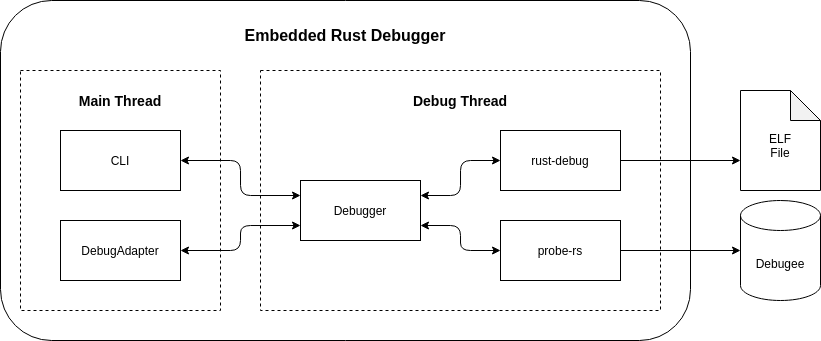
\includegraphics[width=1.0\textwidth]{debugger_structure.png}
    \label{fig:EDBStruct}
\end{figure}


\subsection{Debug Library}
\label{subsection:rust-debug}
\import{implementation/}{debug_library.tex}

\subsection{Debugger}
\import{implementation/}{debugger.tex}

\subsection{Command Line Interface}
\import{implementation/}{cli.tex}

\subsection{Debug Adapter}
\import{implementation/}{debug_adapter.tex}

\subsection{VSCode Extension}
\import{implementation/}{vscode_extension.tex}

